\documentclass[14pt]{beamer} %Makes presentation
%\documentclass[14pt,handout]{beamer} %Makes Handouts
\input{preamble}
\usepackage{tikz}
\usetikzlibrary{shapes,arrows,decorations.pathreplacing}

\title{Statistical Foundations II}

\date[]{}

% noncompliance and intention-to-treat effects


% power and MDE
% panels and attrition
% clustering
% using covariates (briefly)
	% effect heterogeneity
	% blocking/stratification

% lab activity:
	% power calculations
	% ITT, etc.
	% attrition


\begin{document}

\frame{\titlepage}

\frame{\tableofcontents}

\section{Administrative Stuff}
\frame{\tableofcontents[currentsection]}

\frame{

\frametitle{Administrative Stuff}

\begin{enumerate}\itemsep1em
\item<2-> Summative Essay Deadline
	\begin{itemize}
	\item Current: Tuesday MT Week 11
	\item Option A: Tuesday LT Week 1
	\item Option B: Tuesday LT Week 2
	\end{itemize}

\item<3-> Topics for Weeks 6--11?
\end{enumerate}

}



\section{An Example}
\frame{\tableofcontents[currentsection]}


\frame{

\frametitle{Definitions}

\small

\begin{enumerate}\itemsep1em

\item \textbf{Unit}: A physical object at a particular point in time

\item \textbf{Treatment}: An intervention, whose effect(s) we wish to assess relative to some other (non-)intervention

\item \textbf{Outcome}: The variable we are trying to explain

\item \textbf{ATE}: The comparison between average potential outcomes under each intervention

\end{enumerate}

}

\frame{

\frametitle{Banerjee et al}

What are the following in this experiment:

\begin{enumerate}\itemsep1em

\item \textbf{Unit}: ?

\item \textbf{Treatment}: ?

\item \textbf{Outcome}: ?

\item \textbf{ATE}: ?

\end{enumerate}

What else should we know about this experiment?

}








\section{Statistical Inference}
\frame{\tableofcontents[currentsection]}



\frame{

\frametitle{Randomization Inference I}

\begin{itemize}\itemsep1em
\item The randomization (or permutation) distribution is an empirical sampling distribution
\item It conveys the variation we would observe in $\widehat{ATE}$ if a null hypothesis, $H_0: ATE = 0$ was true
\item If this null hypothesis is true, then treatment had no effect; the variation in permuted ATEs therefore only reflects sampling variance
\end{itemize}
}



\frame{

\frametitle{Randomization Distribution}

The randomization distribution is the vector of all possible ATEs that could be observed in the dataset under rerandomization:

\begin{center}
\begin{tabular}{cr}
\texttt{Randomization} & \texttt{ATE} \\ \hline 
1 & 3.25 \\
2 & -1.50 \\
3 & 0.75 \\
4 & \dots \\
\dots & \dots  \\ \hline
\end{tabular}
\end{center}

In a two-condition experiment, the number of possible permutations is given by ${n}\choose{n_1}$.

}


\frame{

\frametitle{Randomization Inference II}

Randomization inference works as follows:

\begin{enumerate}\itemsep0.5em
\item Generate every possible randomization scheme
	\begin{itemize}
	\item Or sample from all possible randomizations
	\end{itemize}
\item Calculate $ATE$ under each randomization
\item The distribution of those estimates is the randomization distribution
\item Its variance is $\widehat{Var}(ATE)$
\item Proportion of values further from 0 than the observed $\widehat{ATE}$ is the p-value for a test of the null hypothesis ($H_0: ATE = 0$)
\end{enumerate}

}

\frame{
\begin{center}
\includegraphics[width=\textwidth]{images/randomization}
\end{center}
}



\begin{frame}[fragile]

\frametitle{Randomization Inference in R}

\footnotesize

\begin{verbatim}
# construct data
d <- data.frame(x = c(0,0,0,0,1,1,1,1), 
                y = c(5,7,9,4,11,4,13,12))

# calculate ATE from each randomization
set.seed(1)    # set random number seed
n <- 10000     # number of randomizations
rd <- replicate(n, coef(lm(d$y ~ sample(d$x, 8)))[2L])

# visualize the randomization distribution
hist(rd)
abline(v = coef(lm(y~x, data = d))[2L], col = "red")

# one-tailed significance test
sum(rd >= coef(lm(y ~ x, data = d))[2L])/n
# two-tailed significance test
sum(abs(rd) >= coef(lm(y ~ x, data = d))[2L])/n
\end{verbatim}

\end{frame}


\begin{frame}[fragile]

\frametitle{Parametric Analysis Stata/R}

R:\small
\begin{verbatim}
t.test(outcome ~ treatment, data = data)
lm(outcome ~ factor(treatment), data = data)
\end{verbatim}

\vspace{1em}

Stata:\small
\begin{verbatim}
ttest outcome, by(treatment)
reg outcome i.treatment
\end{verbatim}

\end{frame}


\frame{\huge\vskip20pt\textbf{Questions?}}



\section{Variance and Power}
\frame{\tableofcontents[currentsection]}


\frame{

\frametitle{Intuition about Variance}

\begin{itemize}\itemsep1em
\item Basic intuition:

	\begin{itemize}
	\item Bigger sample $\rightarrow$ smaller SEs
	\item Smaller variance $\rightarrow$ smaller SEs
	\end{itemize}

\item Other design features also matter

\item Why do we care?
\end{itemize}

}


\frame{

\frametitle{Statistical Power}

\begin{itemize}\itemsep0.5em
\item Power analysis is used to determine sample size before conducting an experiment

\item Type I and Type II Errors

\begin{center}
\begin{tabular}{lcc}
\toprule
& $H_0$ False & $H_0$ True \\ 
& ($|ATE| > 0$) & ($ATE = 0$) \\ \midrule
Reject $H_0$ & \textbf{True positive} & Type I Error \\
Accept $H_0$ & Type II Error & True zero \\ \bottomrule
\end{tabular}
\end{center}

	\begin{itemize}
	\item True positive rate ($1-\kappa$) is power
	\item False positive rate is the significance threshold ($\alpha$)
	\end{itemize}

\end{itemize}
}


\frame{

\frametitle{Doing a Power Analysis}

\begin{itemize}
\item $\mu$, Treatment group mean outcomes
\item $n$, Sample size
\item $\sigma$, Outcome variance
\item $\alpha$ Statistical significance threshold
\item $\phi$, a sampling distribution
\end{itemize}

$Power = 1 - \kappa = \phi\left( \frac{|\mu_1 - \mu_0|\sqrt{n}}{2\sigma} - \phi^{-1}\left( 1 - \frac{\alpha}{2} \right) \right)$

\vspace{1em}

(You don't need to know this formula!)

}



\frame{
\frametitle{Intuition about Power}

Minimum detectable effect is the smallest effect we could detect given sample size, ``true'' ATE, variance of outcome measure, power ($1-\kappa$), and $\alpha$.\\

\vspace{1em}

\only<2->{In essence: some non-zero effect sizes are not detectable by a study of a given sample size.}

\vspace{1em}

\only<3->{In underpowered study, we will be unlikely to detect true small effects. And most effects are small! \footnote{Gelman, A. and Weakliem, D. 2009. ``Of Beauty, Sex and Power.'' \textit{American Scientist} 97(4): 310--16}}

}


\frame{

\frametitle{Intuition about Power}

\begin{itemize}\itemsep1em
\item It can help to think in terms of ``standardized effect sizes''
\item Intuition: How large is the effect in standard deviations of the outcome?
	\begin{itemize}
	\item Know if effects are large or small
	\item Compare effects across studies
	\end{itemize}
\item<2-> Cohen's $d$:\\ $d = \frac{\bar{x}_1 - \bar{x}_0}{s}$, where
$s = \sqrt{\frac{(n_1 - 1)s_1^2 + (n_0 - 1)s_0^2}{n_1 + n_0 - 2}}$
\item<3-> Small: 0.2; Medium: 0.5; Large: 0.8
\end{itemize}

}

\frame{
\frametitle{Intuition about Power}

\begin{center}
\includegraphics[height=0.8\textheight, trim = 0in 0in 0in 0.5in , clip]{images/power}
\end{center}

}


\begin{frame}[fragile]

\frametitle{Power analysis in R I}
\small
\begin{verbatim}
power.t.test(
  # sample size (leave blank!)
  n = ,
  
  # minimum detectable effect size
  delta = 0.4, sd = 1,
  
  # alpha and power (1-kappa)
  sig.level = 0.05, power = 0.8,
  
  # two-tailed vs. one-tailed test
  alternative = "two.sided"
)
\end{verbatim}
\end{frame}

\begin{frame}[fragile]
\frametitle{Power analysis in R II}
\small
\begin{verbatim}
# Given a sample size, what is the MDE?
power.t.test(n = 50, power = 0.8)

# Given a sample size and MDE, what is power?
power.t.test(n = 50, delta = 0.2)

\end{verbatim}
\end{frame}


\frame{}



\begin{frame}

\frametitle{Increasing/Decreasing Power}

\begin{columns}
\begin{column}{0.5\textwidth}
\begin{block}{Increases Power}
\begin{itemize}\itemsep1em
\item Bigger sample
\item Precise measures
\item Covariates?
\end{itemize}
\end{block}
\end{column}

\begin{column}{0.5\textwidth}
\begin{block}{Decreases Power}
\begin{itemize}\itemsep1em
\item Attrition
\item Noncompliance
\item Clustering
\end{itemize}
\end{block}
\end{column}
\end{columns}

\end{frame}


\frame{

\frametitle{Covariates in Experiments}

\begin{itemize}\itemsep1em
\item<2-> Identification of a causal effect only requires randomization
\item<2-> We don't need to include covariates in analysis!

	\begin{align}
	Y & = \beta_0 + \beta_1 X + \epsilon \\
	Y & = \beta_0 + \beta_1 X + \beta_{2-J} Z + \epsilon
	\end{align}

\item<4-> Independence of potential outcomes from treatment assignment is an \textit{asymptotic} property of randomization!
\end{itemize}

}

\frame{

\frametitle{Block Randomization I}

\begin{itemize}\itemsep0.5em
\item<2-> Basic idea: randomization occurs within strata defined \textit{before} treatment assignment
\item<3-> CATE is estimate for each stratum; aggregated to SATE
\item<4-> Why?
	\begin{itemize}
	\item Eliminate chance imbalances
	\item Optimized for estimating CATEs
	\item More precise SATE estimate
	\end{itemize}
\end{itemize}

\onslide<5->{\textbf{Stratification:Sampling::Blocking:Experiments}}


}

\begin{frame}[fragile]

\begin{center}
\begin{tabular}{lcccccccc}
Exp. & \multicolumn{4}{c}{Control} & \multicolumn{4}{c}{Treatment} \\ \midrule
1 & M & M & M & M & F & F & F & F \\
2 & M & M & M & F & M & F & F & F \\
3 & M & M & F & F & M & M & F & F \\
4 & M & F & F & F & M & M & M & F \\
5 & F & F & F & F & M & M & M & M \\ \bottomrule
\end{tabular}
\end{center}

\end{frame}

\frame{

\begin{center}

\begin{tabular}{rrrr}
Obs. & $X_{1i}$ & $X_{2i}$ & $D_i$ \\ \midrule
1 & Male & Old & 0 \\
2 & Male & Old & 1 \\  \midrule
3 & Male & Young & 1 \\
4 & Male & Young & 0 \\ \midrule
5 & Female & Old & 1 \\
6 & Female & Old & 0 \\ \midrule
7 & Female & Young & 0 \\
8 & Female & Young & 1 \\ \bottomrule
\end{tabular}
\end{center}

}

\frame[label=blocking2]{

\frametitle{Block Randomization II}

\begin{itemize}
\item Blocking ensures ignorability of all covariates used to construct the blocks
\item Incorporates covariates explicitly into the \textit{design}
\item<2-> When is blocking \textit{statistically} useful?
	\begin{itemize}
	\item<3-> If those covariates affect values of potential outcomes, blocking reduces the variance of the SATE
	\item<4-> Most valuable in small samples
	\item<5-> Not valuable if all blocks have similar potential outcomes
	\end{itemize}
\end{itemize}

}



\frame{

\frametitle{Statistical Properties I}

\small

Complete randomization:\\
$$SATE = \frac{1}{n_1}\sum Y_{1i} - \frac{1}{n_0}\sum Y_{0i}$$

\vspace{2em}

Block randomization:\\
$$SATE_{blocked} = \sum_{1}^{J} \left( \dfrac{n_j}{n} \right)  (\widehat{CATE}_j)$$

}


\frame{

\begin{center}

\begin{tabular}{rrrrrr}
Obs. & $X_{1i}$ & $X_{2i}$ & $D_i$ & $Y_i$ & CATE \\ \midrule
1 & Male & Old & 0 & 5 & \multirow{2}{*}{\onslide<2->{5}} \\
2 & Male & Old & 1 & 10 \\  \midrule
3 & Male & Young & 1 & 4 & \multirow{2}{*}{\onslide<3->{3}} \\
4 & Male & Young & 0 & 1 \\ \midrule
5 & Female & Old & 1 & 6 & \multirow{2}{*}{\onslide<4->{4}} \\
6 & Female & Old & 0 & 2 \\ \midrule
7 & Female & Young & 0 & 6 & \multirow{2}{*}{\onslide<5->{3}} \\
8 & Female & Young & 1 & 9 \\ \bottomrule
\end{tabular}
\end{center}

}

\frame{

\frametitle{SATE Estimation}

\begin{align*}
SATE &= \left(\dfrac{2}{8}*5\right) + \left(\dfrac{2}{8}*3\right) + \left(\dfrac{2}{8}*4\right) + \left(\dfrac{2}{8}*3\right) \\ \vspace{1em}
&= 3.75
\end{align*}

\onslide<2->{The blocked and unblocked estimates are the same here because $Pr(Treatment)$ is constant across blocks and blocks are all the same size.}

}

\frame{

\frametitle{SATE Estimation}

\small

\begin{itemize}
\item We can use weighted regression to estimate this in an OLS framework
\item Weights are the inverse prob. of being treated w/in block
\begin{itemize}
\item Pr(Treated) by block: $p_{ij} = Pr(D_i = 1 | J=j) $
\item Weight (Treated): $ w_{ij} = \dfrac{1}{p_{ij}} $
\item Weight (Control): $ w_{ij} = \dfrac{1}{1-p_{ij}} $
\end{itemize}
\end{itemize}

}


\frame{

\frametitle{Statistical Properties II}

\small

Complete randomization:\\
$$\widehat{SE}_{SATE} = \sqrt{\dfrac{\widehat{Var}(Y_0)}{n_0} + \dfrac{\widehat{Var}(Y_1)}{n_1}}$$

\vspace{1em}

Block randomization:\\
$$\widehat{SE}_{SATE_{blocked}} = \sqrt{\sum_{j=1}^{J} \left( \dfrac{n_j}{n} \right)^2  \widehat{Var}{(CATE_j)}}$$

\only<2->{When is the blocked design more efficient?}

}


\frame{\huge\vskip20pt\textbf{Questions?}}


\frame{

\frametitle{Baseline Outcome Measure}

\begin{itemize}\itemsep0.5em
\item Recall our key definition:
\end{itemize}

	\begin{quote}\small
		The observation of units after, \textbf<2->{and possibly before}, a randomly assigned intervention in a controlled setting, which tests one or more precise causal expectations
	\end{quote}

\begin{itemize}\itemsep0.5em

\item<3-> Pretreatment measures of the outcome can be particularly helpful!

\end{itemize}
}

\frame{

\frametitle{Baseline Outcome Measure}

\begin{itemize}\itemsep0.5em
\item<1-> This changes our estimator of $ATE$ from simple \textit{mean-difference} to \textit{difference-in-differences} (DID)

	\begin{align*}
	(\hat{Y}_{0,t+1} - \hat{Y}_{0,t}) - (\hat{Y}_{j,t+1} - \hat{Y}_{j,t})
	\end{align*}

\item Advantageous because variance for paired samples decreases as correlation between $Y_0$ and $Y_1$ increases
\end{itemize}

}

\frame{
	\begin{center}
	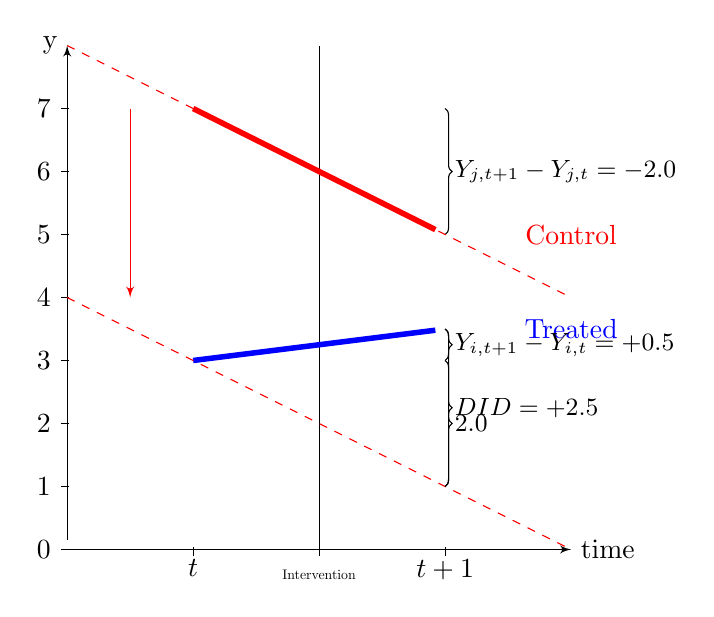
\begin{tikzpicture}[>=latex', scale=0.8]
        \draw[->] (0,0) node (origin) {}  -- (8,0) node[right] (xaxis) {time};
        \draw[->] (origin) -- (0,8) node[left] (yaxis) {y};
        % x ticks
        \foreach \x in {2,4,6}
        	\draw (\x,1pt) -- (\x,-3pt) node[anchor=north] {};
        \draw (2,0) node[below] (before) {$t$};
        \draw (6,0) node[below] (after) {$t+1$};
        \draw (4,-0.25) node[below, scale=0.5] (IV) {Intervention};
        % y ticks
        \foreach \y in {0,...,7}
             \draw (1pt,\y) -- (-3pt,\y) node[anchor=east] {$\y$};
        % intervention
        \draw (4,0) -- (4,8);

        % line
        \draw<2-> (6,3.5) node (tr) {};
        \draw<3-> (6,5) node (ctrl) {};
        \draw<2-3>[blue] (8,3.5) node (trlab) {Treated};
        \draw<3-3>[red] (8,5) node (ctrllab) {Control};        
        \draw<2->[blue, line width=2pt] (2,3) -- (tr);
        \draw<3->[red, line width=2pt] (2,7) -- (ctrl);
        
        % diffs
        \draw<4-6>[right,decorate,decoration={brace,mirror}] 
        	(6,3) -- (6,3.5) node[right, pos=0.5] (idiff) {\small $Y_{i,t+1} - Y_{i,t} = +0.5$};
        \draw<4-6>[right,decorate,decoration={brace}] 
            (6,7) -- (6,5) node[right, pos=0.5] (jdiff) {\small $Y_{j,t+1} - Y_{j,t} = -2.0$};
        
        % trends
        \draw<5-6>[red,->] (1,7) -- (1,4);
        \draw<5->[red, dashed] (0,8) -- (8,4);
        \draw<5->[red, dashed] (0,4) -- (8,0);
        \draw<6>[right,decorate,decoration={brace}] 
            (6,3) -- (6,1) node[right, pos=0.5] (idiff2) {\small $2.0$};
        \draw<7>[right,decorate,decoration={brace}] 
            (6,3.5) -- (6,1) node[right, pos=0.5] (idiff2) {\small $DID = +2.5$};
                        
        
    \end{tikzpicture}
    \end{center}
}


\begin{frame}
\frametitle{Statistical Advantages I}	

In post-treatment-only designs:

\begin{equation*}
\widehat{ATE}_{Diff} = \dfrac{\sum_{i=1}^{n_1} (x_{i,1,t+1})}{n_1} - \dfrac{\sum_{i=1}^{n_0} (x_{i,0,t+1})}{n_0}
\end{equation*}

The variance of this estimate is:

\begin{align*}
Var(\widehat{ATE}_{Diff}) &=  Var(\bar{Y}_{1,t+1}) + Var(\bar{Y}_{0,t+1})%\\
%&= \dfrac{\frac{1}{n_1}\sum_{i=1}^{n_1} (x_{i,1} -\bar{x}_1)^2}{n_1} + \dfrac{\frac{1}{n_0}\sum_{i=1}^{n_0} (x_{i,0} -\bar{x}_1)^2}{n_0}
\end{align*}
\end{frame}

\frame{
\frametitle{Statistical Advantages II}

In pre/post-treatment designs:

\begin{equation*}
\widehat{ATE}_{DID} = \dfrac{\sum_{i=1}^{n_1} (x_{i,1,t+1} - x_{i,1,t})}{n_1} - \dfrac{\sum_{i=1}^{n_0} (x_{i,0,t+1} - x_{i,0,t})}{n_0}
\end{equation*}

The variance of this estimate is:

\small

\begin{align*}
Var(\widehat{ATE}_{DID}) &=  Var(\bar{Y}_{1,t+1} - \bar{Y}_{1,t}) + Var(\bar{Y}_{0,t+1} - \bar{Y}_{0,t}) \\
&= \left(Var(\bar{Y}_{1,t+1}) + Var(\bar{Y}_{1,t}) - Cov(\bar{Y}_{1,t+1}, \bar{Y}_{1,t})\right) \\
&+ \left(Var(\bar{Y}_{0,t+1}) + Var(\bar{Y}_{0,t}) - Cov(\bar{Y}_{0,t+1}, \bar{Y}_{0,t}) \right)
\end{align*}

}



\begin{frame}[fragile]

\small

\begin{verbatim}
# create some fake data
set.seed(54321)
n <- 400L
y0 <- rnorm(n)
x <- rbinom(n, 1L, 0.5)

# high Cor(y0, y1)
y1a <- y0 + 0.25*x + rnorm(n, sd = 0.25)
summary(lm(y1a ~ x))
summary(lm(I(y1a-y0) ~ x))

# low Cor(y0, y1)
y1b <- y0 + 0.25*x + rnorm(n, sd = 2)
summary(lm(y1b ~ x))
summary(lm(I(y1b-y0) ~ x))
\end{verbatim}

\end{frame}



\frame{

\frametitle{Practicalities}

\begin{itemize}\itemsep1em
\item Blocked randomization and use of pre-treatment measures only works in some circumstances

\item Need to observe covariates pre-treatment in order to block on them

	\begin{itemize}
	\item Challenging in a cross-sectional design
	\end{itemize}

\item The cost of gathering pre-treatment data might also outweigh the gain in precision

	\begin{itemize}
	\item May introduce other biases
	\end{itemize}

\end{itemize}

}


\frame{\huge\vskip20pt\textbf{Questions?}}

\frame{

\frametitle{Clustering}

\begin{itemize}\itemsep0.5em
\item Everything so far assumes units are \textit{independent}
\item Sometimes units are obviously not independent
	\begin{itemize}
	\item e.g., Students within classrooms
	\end{itemize}
\item Non-independence limits our ability to randomize at the unit level and reduces statistical power
\end{itemize}

}




\appendix
\frame{}

\end{document}
